\chapter{Alternating Current}

We have discussed the voltage and current created by a battery.  A
battery pushes the electrons in one direction at a constant voltage;
this is known as \newterm{Direct Current} or DC. A battery typically
provides between 1.5 and 9 volts.

The electrical power that comes into your home on wires is
different. If you plotted the voltage over time, it would look like
this:
\begin{figure}[htbp]
    \centering
      \begin{tikzpicture}[
      tl/.style = {% tick labels fill=white, inner sep=1pt,
        font=\scriptsize, }, ]
      % grid
      \draw[sdkblue, very thin, xstep=0.5235, ystep=0.425] (0,-1.85) grid
      (6.6,1.85);
      
      % y tick label
      \foreach \y in {-170, -85, 85, 170}{\node[tl,left=1mm] at (0,{\y/100})
        {$\y$};}
      
      % x tick label
      \foreach \x in {0.004,0.008, 0.012, 0.016}{\node[tl,below=1mm] at
        ({392.67*\x},0) {$\x$};}
      
      % axes
      \draw[->,thick] (0,0) -- (6.5,0) node[right] {$seconds$};
      \draw[->,thick] (0,-1.8) -- (0, 1.8) node[above] {$volts$};
      % curve
      \draw[<->,thick,draw=black,domain=0:6.5,samples=300,variable=\x] plot
      (\x,{sin(deg(\x)) * 1.7});
      \end{tikzpicture}
    \caption{A graph of AC voltage over time.}
    \label{fig:acvoltsGraph}
\end{figure}

The $x$ axis here represents ground. When you insert a two-prong plug
into an outlet, one is ``hot'' and the other is ``ground''. Ground
represents 0 volts and should be the same voltage as the dirt under
the building.

The voltage is a sine wave at 60Hz. Your voltage fluctuates between
-170v and 170v. Think for a second what that means: The power company
pushes electrons at 170v, then pulls electrons at 170v.  It
alternates back and forth this way 60 times per second.

\section{Power of AC}

Let's say you turn on your toaster, which has a resistance of 14.4
ohms. How much energy (in watts) does it change from electrical energy
to heat? We know that $I = V/R$ and that watts of power are
$IV$. So, given a voltage of $V$, the toaster is consuming $V^2/R$
watts.

However, $V$ is fluctuating. Let's plot the power the toaster is consuming:
\begin{figure}[htbp]
    \centering
    \begin{tikzpicture}[
    tl/.style = {% tick labels
        fill=white, inner sep=1pt, font=\scriptsize,
                },                        ]
    % grid
    \draw[sdkblue, very thin, xstep=0.5235, ystep=0.5] (0,0) grid (6.6,2.1);
    
    % y tick label
    \foreach \y in {500, 1000, 1500, 2000}{\node[tl,left=1mm] at (0,{\y/1000}) {$\y$};}
    
    % x tick label
    \foreach \x in {0.004,0.008, 0.012, 0.016}{\node[tl,below=1mm] at ({392.67*\x},0) {$\x$};}
    
    % axes
    \draw[->,thick] (0,0) -- (6.5,0) node[right] {$seconds$};
    \draw[->,thick] (0,0) -- (0, 2.1) node[above] {$watts$};
    % curve
    \draw[<->,thick,draw=black,domain=0:6.5,samples=300,variable=\x]
          plot (\x,{sin(deg(\x))^2 * 2.007});
    \end{tikzpicture}
    \caption{A plot of AC power over time.}
    \label{fig:acpowerGraph}
\end{figure}

Another sine wave! Here is a lesser-known trig identity: $\left( \sin(x) \right)^2 = \frac{1}{2} - \frac{1}{2}\cos(2x)$

This is actually a cosine wave flipped upside down, scaled down by
half the peak power, and translated up so that it is never
negative. Note that it is also twice the frequency of the voltage sine
wave.

If we say the peak voltage is $V_p$ and the resistance of the toaster
is $R$, the power is given by

$$\frac{V_p^2}{2R} - \frac{V_p^2}{2R} \cos \left(\frac{2\pi t}{120} \right)$$

As a toaster user and as someone who pays a power bill, you are mostly
interested in the average power.  To get the average power, you take
the area under the power graph and divide it by the amount of time.

We can think of the area under the curve as two easy-to-integrate quantities summed:
\begin{itemize}
\item A constant function of $y = frac{V_p^2}{2R}$
\item A wave $y = - \frac{V_p^2}{2R} \cos \left(\frac{2\pi t}{120} \right)$
\end{itemize}

\begin{tikzpicture}[
tl/.style = {% tick labels
    fill=white, inner sep=1pt, font=\scriptsize,
            },                        ]
% grid
\draw[sdkblue, very thin, xstep=0.5235, ystep=0.5] (0,-1.1) grid (6.6,1.1);

% y tick label
\foreach \y in {-1000, -500, 500, 1000}{\node[tl,left=1mm] at (0,{\y/1000}) {$\y$};}

% x tick label
\foreach \x in {0.004,0.008, 0.012, 0.016}{\node[tl,below=1mm] at ({392.67*\x},0) {$\x$};}

% axes
\draw[->,thick] (0,0) -- (6.5,0) node[right] {$seconds$};
\draw[<->,thick] (0,-1.1) -- (0, 1.1) node[above] {$watts$};
% curve
\draw[<->,thick,draw=black] (0,1.003) -- (6.5, 1.003) node[right] {Constant: $\frac{V_p^2}{2R}$};
\draw[<->,thick,draw=black,domain=0:6.5,samples=300,variable=\x]
      plot (\x,{-1 * cos(deg(\x) * 2) * 1.003}) node[right]{Wave:$- \frac{V_p^2}{2R} \cos \left(\frac{2\pi t}{120} \right)$};
\end{tikzpicture}
    
When we integrate that constant function, we get $\frac{t V_p^2}{2R}$.

When we integrate that wave for a complete cycle we get...zero! The
positive side of the wave is canceled out by the negative side.

So, the average power is $\frac{V_p^2}{2R}$ watts.

Someone at some point said, ``I'm used to power being $V^2/R$. Can
we define a voltage measure for AC power such that this is always true?''

So we started using $V_{rms}$ which is just
$\frac{V_p}{\sqrt{2}}$. If you look on the back of anything that plugs
into a standard US power outlet, it will say something like ``For
120v''.  What they mean is, ``For 120v RMS, we expect the voltage to
fluctuate back and forth from 170v to -170v.''

Notice that this is the same Root-Mean-Squared that we defined
earlier, but now we know that if $y = \sin(x)$, the RMS of $y$ is
$1/\sqrt{2} \approx 0.707$.

For current, we do the same thing. If the current is AC, the power
consumed by a resistor is $I_{RMS}^2 R$, where $I_{RMS}$ is the peak
current divided by $\sqrt{2}$.

\section{Power Line Losses}

A wire has some resistance. Thinner wires tend to have more resistance
than thicker ones. Aluminum wires tend to have more resistance than
copper wires.

Let's say that the power that comes to your house has to travel 20 km
from the generator in a cable that has about $1 \Omega$ of resistance
per km.  Let's also say that your home is consuming 12 kilowatts of power.

If that power is 120v RMS from the generator to your home, what
percentage of the power is lost heating the power line? 10 amps RMS
flow through your home. When that current goes through the wire, $I^2
R = (100)(20) = 2000 \text{ watts}$ is lost to heat.

This means the power company would need to supply 14 kilowatts of power,
knowing that 2 kilowatts would be lost on the wires.

What if the power company moved the power at 120,000 volts RMS? Now
only 0.01 amps RMS flow through your home. When that current goes
through the wire $I^2R = (0.0001)(20) = .002$ watts of power are lost
on the power lines.

This is much, much more efficient. The only problem is that 120,000 volts
would be incredibly dangerous.  So the power company moves power long
distances at very high voltages, like 765 kV.  Before the power is
brought into your home, it is converted into a lower voltage using a
\newterm{transformer}.

\section{Transformers}

A transformer is a device that converts electrical power from one
voltage to another. A good transformer is more than 95\% efficient. The
details of magnetic fields, flux, and inductance are beyond the scope
of this chapter, so we are going to give a relatively simple (and admittedly incomplete) explanation for now.

A transformer is a ring with two sets of coils wrapped around it.
\begin{figure}[htbp]
    \centering
    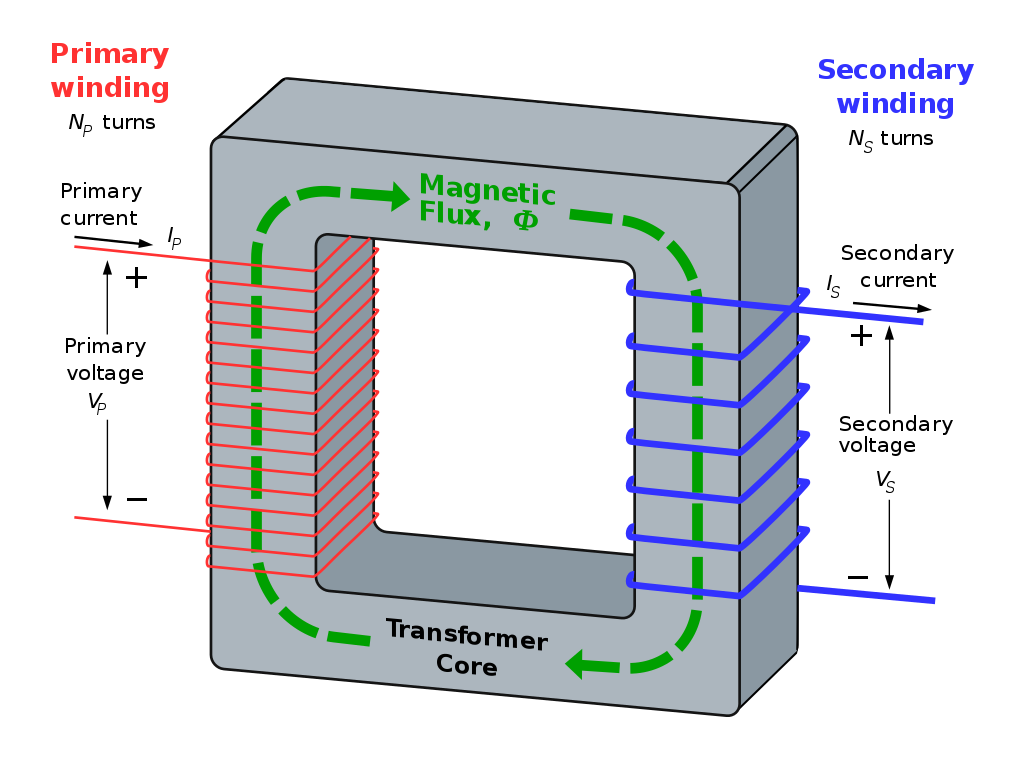
\includegraphics[width=0.5\textwidth]{transformer.png}
    \caption{A diagram of a transformer from Wikipedia.}
    \label{fig:transformer}
\end{figure}

When alternating current is run through the primary winding, it creates magnetic
flux in the ring. The magnetic flux induces current in the secondary
winding.

If $V_P$ is the voltage across the primary winding and $V_S$ is the
voltage across the secondary winding, they are related by the
following equation:

$$\frac{V_P}{V_S} = \frac{N_P}{N_S}$$

where $N_P$ and $N_S$ are the number of turns in the primary and
secondary windings.

There are usually at least two transformers between you and the very
high voltage lines. There are transformers at the substation that make
the voltage low enough to travel on regular utility poles. On the
utility poles, you will see cans that contain smaller
transformers. Those step the voltage down to make the power safe to
enter your home.

\section{Phase and 3-phase power}

If two waves are ``in sync'', we say they have the same \newterm{phase}.
\begin{figure}[htbp]
    \centering
    \begin{tikzpicture}[
    tl/.style = {% tick labels fill=white, inner sep=1pt,
      font=\scriptsize, }, ]
    % grid
    \draw[sdkblue, very thin, xstep=0.5235, ystep=0.425] (0,-1.85) grid
    (13,1.85);
    
    % axes
    \draw[->,thick] (0,0) -- (13,0);
    % curve
    \draw[thick,draw=black,domain=0:13,samples=500,variable=\x] plot
    (\x,{sin(deg(\x)) * 1.7});
    \draw[thick,dashed, draw=black,domain=0:13,samples=500,variable=\x] plot
    (\x,{sin(deg(\x)) * 0.9});
    \end{tikzpicture}
    \caption{A diagram of two AC signals in sync.}
    \label{fig:ACsync}
\end{figure}

If they are the same frequency, but are not in sync, we can talk about
the difference in their phase.
\begin{figure}[htbp]
    \centering
    \begin{tikzpicture}[
    tl/.style = {% tick labels fill=white, inner sep=1pt,
      font=\scriptsize, }, ]
    % grid
    \draw[sdkblue, very thin, xstep=0.5235, ystep=0.425] (0,-1.85) grid
    (13,1.85);
    
    % axes
    \draw[->,thick] (0,0) -- (13,0);
    % curve
    \draw[thick,draw=black,domain=0:13,samples=500,variable=\x] plot
    (\x,{sin(deg(\x)) * 1.7});
    \draw[thick,dashed, draw=black,domain=0:13,samples=500,variable=\x] plot
    (\x,{sin(deg(\x) - 90) * 0.9});
    \end{tikzpicture}
    \caption{A diagram of two AC signals out of phase.}
    \label{fig:ACoutsync}
\end{figure}

Here, we see that the smaller wave is lagging by $\pi/2$ or $90^\circ$.

In most power grids, there are usually three wires carrying the power.
The voltage on each is $2\pi/3$ out of phase with the other two:
\begin{figure}[htbp]
    \centering
    \begin{tikzpicture}[
    tl/.style = {% tick labels fill=white, inner sep=1pt,
      font=\scriptsize, }, ]
    % grid
    \draw[sdkblue, very thin, xstep=0.5235, ystep=0.425] (0,-1.85) grid
    (13,1.85);
    
    % axes
    \draw[->,thick] (0,0) -- (13,0);
    % curve
    \draw[thick,draw=black,domain=0:13,samples=500,variable=\x] plot
    (\x,{sin(deg(\x)) * 1.7});
    \draw[thick,dashed, draw=black,domain=0:13,samples=500,variable=\x] plot
    (\x,{sin(deg(\x) - 120) * 1.7});
    \draw[thick,draw=sdkblue,domain=0:13,samples=500,variable=\x] plot
    (\x,{sin(deg(\x) + 120) * 1.7});
    \end{tikzpicture}
    \caption{A diagram of three AC signals, each $2\pi/3$ radians out of phase.}
    \label{fig:ACphase}
\end{figure}

This is nice in two ways:
\begin{itemize}
\item While the power in each wire is fluctuating, the total power is not fluctuating at all.
\item While the power plant is pushing and pulling electrons on each
  wire, the total number number of electrons leaving the load is zero.
\end{itemize}
(Both these assume that there each wire is attached to a load with the same constant resistance.)

In big industrial factories, you will see all three wires enter the
building. Large amounts of smooth power delivery means a great deal to an
industrial user.

In residential settings, each home gets its power from one of the three
wires. However, two wires typically carry power into the home. Each
one carries 120V RMS, but they are out of phase by 180 degrees. Lights
and small appliances are connected to one of the wires and ground, so
they get 120V RMS. Large appliances, like air conditioners and
washing machines, are connected across the two wires, so they get 240V
RMS.

\begin{figure}[htbp]
    \centering
    \begin{tikzpicture}[
    tl/.style = {% tick labels fill=white, inner sep=1pt,
      font=\scriptsize, }, ]
    % grid
    \draw[sdkblue, very thin, xstep=0.5235, ystep=0.425] (0,-1.85) grid
    (13,1.85);
    
    % axes
    \draw[->,thick] (0,0) -- (13,0);
    % curve
    \draw[thick,draw=black,domain=0:13,samples=500,variable=\x] plot
    (\x,{sin(deg(\x)) * 1.7});
    \draw[thick,dashed, draw=black,domain=0:13,samples=500,variable=\x] plot
    (\x,{sin(deg(\x) + 180) * 1.7});
    \draw[<->, thick, draw=black] (7.85398, 0) -- (7.85398, 1.7) node [midway, right] {120V};
    \draw[<->, thick, draw=black] (4.712, -1.7) -- (4.712, 1.7);
    \draw (4.712, 0.8) node[right] {240V};
    \end{tikzpicture}
    \caption{A diagram of AC out of phase in homes.}
    \label{fig:AChomephase}
\end{figure}


How do you get two circuits, 180 degrees out of phase, from one
circuit?  Using a center-tap transformer.

FIXME: Diagram here




